\section{COACHES Environment, Hardware and Software Architecture}
\vspace{-0.1cm}
\begin{figure}[t!]
\centering
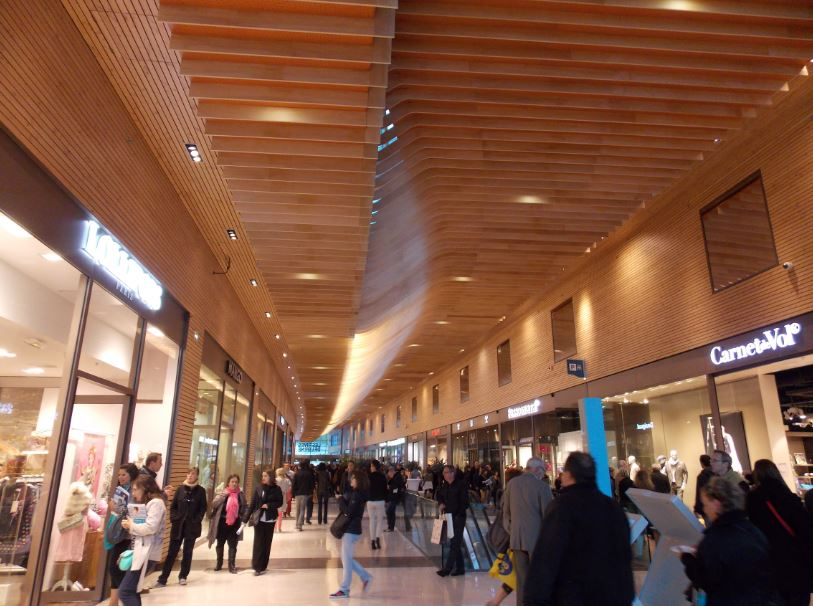
\includegraphics[height=4.2cm]{fig/rivedelorne}\hspace{0.1cm}\hfill
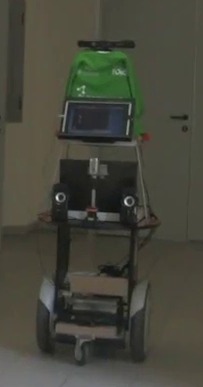
\includegraphics[width=0.18\textwidth]{fig/diago1}\hspace{0.1cm}\hfill
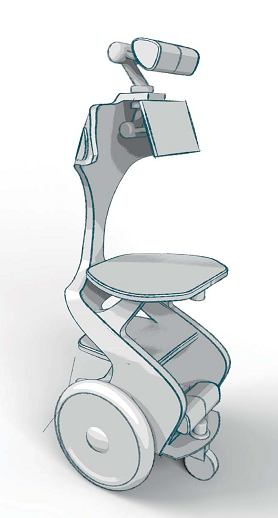
\includegraphics[width=0.18\textwidth]{fig/coaches_robot}
\caption{\coaches environment and robots.}
\label{fig:env}
\end{figure}

In the \coaches project, we aim at further developing this technology, but specifically study, develop and test integration of Artificial Intelligence and Robotics technology in order to develop robots that can suitable interact with users in a complex large public environment, like a shopping mall.
Figure \ref{fig:env} shows, on the left, the \emph{Rive de l'orne} shopping mall in Caen (France) where the experimental activities of the project will be carried out, on the middle a prototype of the robot that will be used for the preliminary experiments and, on the right, the design of the robots that will be realized in Fall 2015.

As shown in the figure, in contrast with previous work on social robotics and human-robot interaction, the \coaches environment is very challenging, because populated by many people.
Moreover, we aim at a more sophisticated interaction using multiple modalities (speech, gesture, touch user interfaces) and dialog generated on-line according to the current situation
and the robot's goals.
Consequently, the required level of ``intelligence'' of the \coaches robots in order to adequately perform complex and effective tasks in this environment in presence of people is much higher than in previous projects.
The \coaches project (October 2014 - September 2017) will provide important insights for actual deployment of intelligent social robots in large populated public areas. 


%\subsection{Software Architecture}

\begin{figure}[t!]
\centering
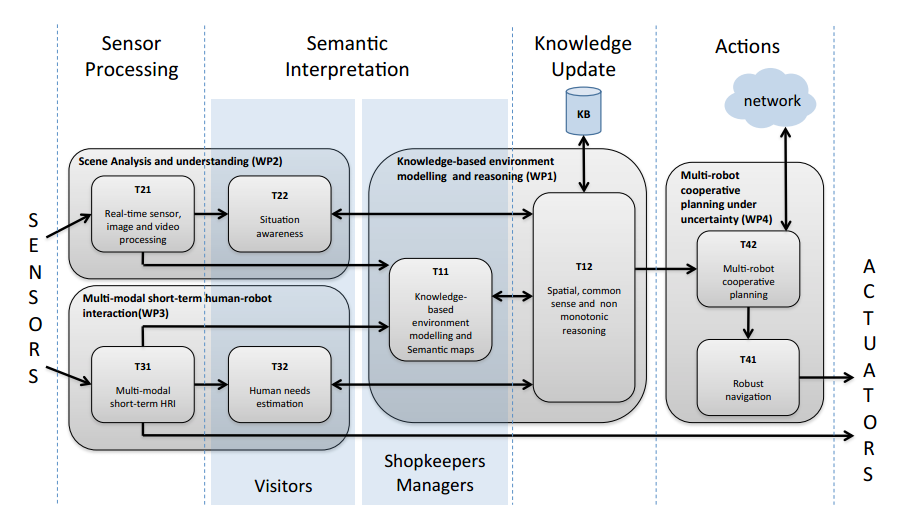
\includegraphics[width=0.95\textwidth]{fig/COACHES_swarch.png}
\caption{\coaches software architecture}
\label{fig:swarch}
\end{figure}

The software architecture of the \coaches robots is shown in Figure \ref{fig:swarch}.
An open architecture (hard/soft) and standard technologies available will be used, 
so that it will be easy to extend and/or adapt the capabilities of the system during the whole length of 
the  project  (especially  to  integrate  and  test  various  algorithms  and/or  sensors).  
Such an open architecture will also simplify and optimize integration efficiency as well as re-use of assets in other projects or products. 


For the development of the robotic software components, the Robot Operating System (ROS)\footnote{www.ros.org}, which is the standard middleware for robotics applications, has been selected.
ROS provides the middleware infrastructure to effectively share information among the many modules implementing various functionalities on each robot. Moreover, an interface (ROS-through-TCP) will be realized in order to share information among the robots and between ROS and non-ROS components of the system.

The main software components that will be developed for control, reasoning and interaction functionalities of the system are listed below.

\vspace{-1em}
\begin{itemize}
\item \emph{Scene analysis}, including sensor processing procedures for both on-board robot devices and static sensors in order to determine the current situation and understand events that are of interest for the system.

\item \emph{Multi-modal HRI}, defining a set of modalities for human-robot interaction, including speech recognition and synthesis, touch interaction, graphical interface on a screen mounted on the robot and Web interfaces.

\item \emph{Knowledge-based representation and reasoning}, defining the formalism and the procedure to represent and reason about the environment and the task of the robots.

\item \emph{Planning and execution monitoring}, for generating the plans to achieve the desired goals and monitor their execution for robust behaviors.

\item \emph{Safe navigation}, for guaranteeing safety operations of the robot in a populated environment.

\end{itemize}

In the next section we will describe the \emph{Short-Term Multi-Modal HRI} component
and, in particular, we show our approach to personalized interactions with users of the shopping mall.

